\section{AHB-Lite PLIC}

The Roa Logic AHB-Lite PLIC (Platform Level Interrupt Controller) IP is a fully parameterized soft IP implementing a Interrupt Controller as specified by the \emph{\href{https://people.eecs.berkeley.edu/\%7Ekrste/papers/riscv-privileged-v1.9.1.pdf}{RISC-V Privileged v1.9.1 specification}}.

The IP features an AHB-Lite Slave interface, with all signals defined in the \emph{\href{https://www.arm.com/products/system-ip/amba-specifications}{AMBA 3 AHB-Lite v1.0}} specifications fully supported. Bus address \& data widths as well as the number of Interrupt Sources and Targets supported are specified via parameters.

The controller further supports user defined priority levels and pending events, in addition to interrupt masking via programmable priority thresholds

\begin{figure}[h]
  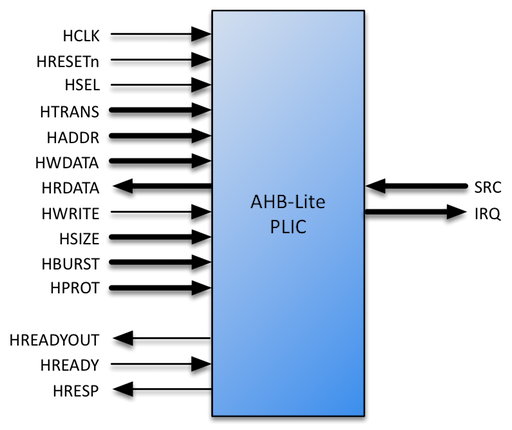
\includegraphics{../assets/graphics/AHB-Lite_PLIC_Port_Diagram.png}
  \caption{PLIC Port Diagram}
  \label{fig:PORTDIAG}
\end{figure}

\subsection{Features}

\begin{itemize}
\item
  AHB-Lite Interface with programmable address and data width
\item
  User defined number of Interrupt Sources \& Targets
\item
  User defined priority level per Interrupt Source
\item
  Interrupt masking per target via Priority Threshold support
\item
  User defined Interrupt Pending queue depth per source
\end{itemize}